% BROKEN labels : section_preparation, section_modeling, section_simulation

\section{Experiments}\label{section_experiments}

%TODO : describe about this section

.. To verify and measure constants of the model discussed in section \ref{section_thermo_model}, two kinds of experiments were carried out - static, and dynamic experiment.

% and verified by three kinds of experiments. 

\subsection{Forced Air Cooling of the SCP Artificial Muscles}\label{section_electrical_control}

In terms of cooling artificial muscles, water and forced air are considered to be a natural method in operating temperature \cite{madden}.
%Even if \scp can be naturally cooled, but natural cooling speed isn't fast enough.
But, water cooling is not appropriate for electrically conductive SCPs. Accordingly, forced air cooling was utilized by using compressed air can.
Muscles was surrounded by cylindric tube to make the air directly flow through the muscles.
This tube was made by thin, plastic tube to minimize the effect on specific heat of the muscles.


%\subsection{Physical Measurements of the SCP Artificial Muscles}
\subsection{Experimental Apparatuses} \label{section_appa}

Physical properties of the \scpsnospace, such as temperature, length, and tension, were measured with various sensors.
\footnote{For the detailed information of sensors, see Table \ref{used_materials}.}
SMD type temperature sensor was used to measure the temperature of \scps without effecting the specific heat of the \scpnospace.

Also, a slide potentiometer was utilized to measure the linear displacement of the \scpsnospace. However, since it had significant amount of friction, it was used when investigating about \scpnospace's characteristics. On the other hand, rotary sensor, which has low frictional torque, was employed to make an \antanospace. 

To measure the tension of the \scpsnospace, a load cell and an amplifier were used.
The load cell played a role in connecting the \scps and the skeleton of the \antanospace.


% TODO : The sentence below is VERY unappropriate for science research paper. This is not a book.
Now let's consider two of the following experimental setup - we will call them as `Setup 1' and `Setup 2', respectively. Setup 1 is 
%
an E-shaped holder that holds each side of the \scp to maintain a constant length which can be customized. (Figure \ref{static_sch}) Additionally, a load cell, a temperature sensor, and a slide potentiometer were used to measure tension, temperature, and length of the \scpnospace, respectively. Also, voltage between muscles was measured to calculate the applied power of the muscle. These sensors were all connected to NI cRIO-9024 for the synchronized real-time data acquisition.

Setup 2 is, 
%
as shown in figure \ref{dynamic_sch}, an air can, a solenoid valve, and a tube which surround actuator were connected in sequence. 
The tube was made with a thin $\SI{4.5}{\centi\meter} \times \SI{12}{\centi\meter}$ plastic layer, in order to minimize the effect on $C_{th}$ of the \scpnospace.
A load was suspended on the end in order to prevent the muscle from becoming loose. 
Also, the temperature sensor was tightly attached to the muscle, and connected to Arduino Uno for the synchronized real-time data acquisition.

%From now on, we will call these setups as `Setup 1' and `Setup 2'.

\begin{figure}[t]
	\centering
	\begin{subfigure}[t]{0.22\textwidth}
		\centering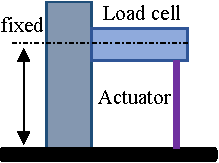
\includegraphics[width=\textwidth]{modeling_static_v2-cropped_compatible.pdf}
		%\centering\includegraphics[width=\textwidth]{example-image-a}
		\caption{\label{static_sch}}
	\end{subfigure}
	\begin{subfigure}[t]{0.22\textwidth}
		\centering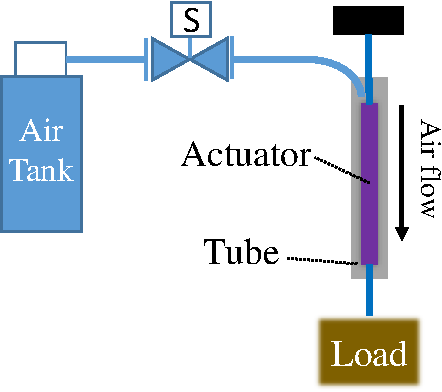
\includegraphics[width=\textwidth]{Static2(v2)_v4-cropped_compatible.pdf}
		\caption{\label{dynamic_sch}}
	\end{subfigure}
	\caption[Scheme of two experimental setups]{\subref{static_sch} Scheme of the `Setup 1'. \subref{dynamic_sch} Scheme of the `Setup 2'.}
	\label{exp_sch}
\end{figure}



Finally, an \anta - which was previously discussed in section \ref{subsection_anta} - was made with two \scpsnospace, which can produce stronger force in two positions within a short time than a single \scpnospace.
First, we made a skeleton of the \anta with 3D printer. (Figure \ref{3d_assemblies}) Then, non-elongating wire was used to connect stand, muscle, and ball bearing with a rotary sensor inside. A cooling device was also attached to the two \scpsnospace. Lastly, sensors of \anta were connected to Arduino Uno with PCB. (Figure \ref{anta_overall})

% TODO : More detailed description

\begin{figure}[t]
	\centering
	\begin{subfigure}[t]{0.3\textwidth}
		\centering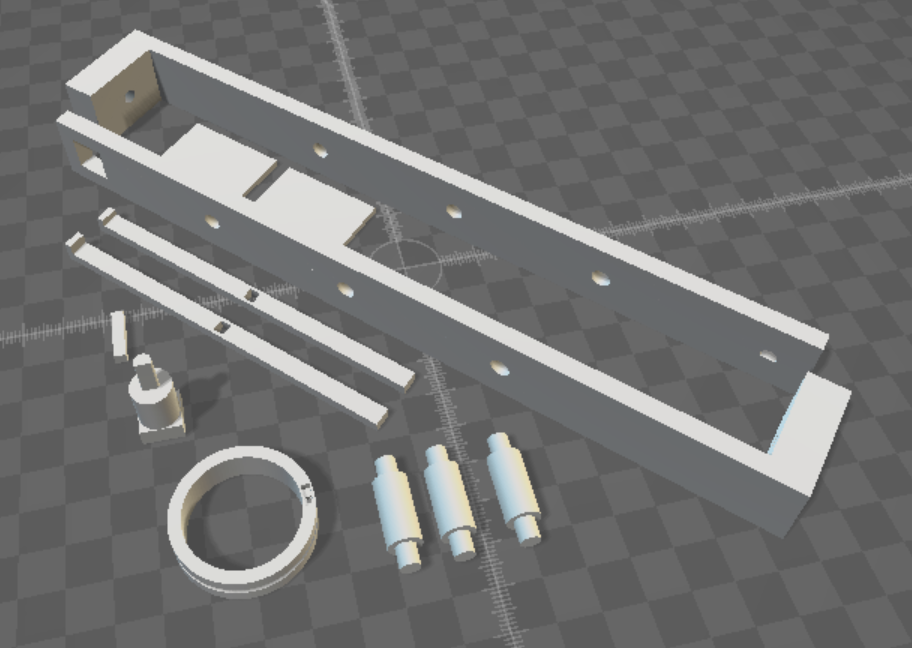
\includegraphics[width=\textwidth]{Anta_3d_assemblies_v2.png}
		\caption{\label{3d_assemblies}}
	\end{subfigure}
	
	\begin{subfigure}[t]{0.81\textwidth}
		\centering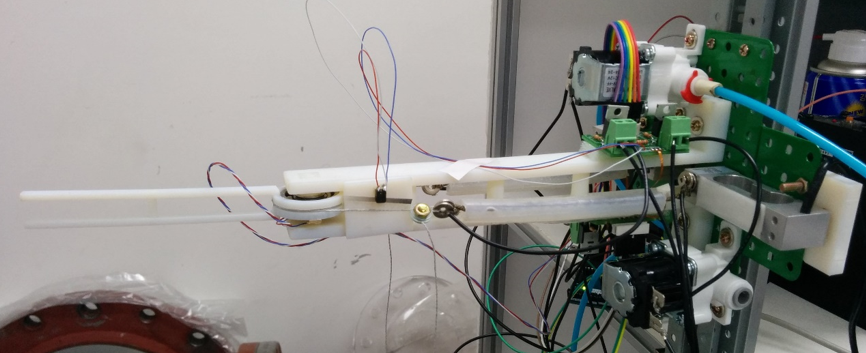
\includegraphics[width=\textwidth]{Anta_overall_v2.png}
		\caption{\label{anta_overall}}
	\end{subfigure}
	
	\caption[\Anta]{\subref{3d_assemblies} The skeleton of the \anta was designed with the software(3D Builder, Microsoft) and 3d-printed. \subref{anta_overall} An overall image of the \anta was as above.}
	\label{anta_design}
\end{figure}

\subsection{Static Experiment} \label{subsection_static_experiment}
The aim of the static experiment was to verify equation \eqref{thermo-mechanical_model}.
First, we checked that muscle's tension changes linearly according to the length, and observed a bit of hysteresis caused by $\dot{x}$.
Then, correlation of the \scpnospace's length and the tension was investigated at various temperatures. 
For this experiment, `Setup 1' was used, which was previously described in \ref{section_appa}.

It can be said that muscles have a length $l_{0}$ at ambient temperature with \SI{0}{\newton} tension. Taking $l_{0}$ as standard, experiments were conducted by changing length \SI{15}{\milli\meter} gradually. Also, five kinds of voltage were used - \SI{0}{\volt}, \SI{1.0}{\volt}, \SI{1.8}{\volt}, \SI{2.2}{\volt}, and \SI{2.6}{\volt}. 
Following processes were carried out.

\begin{enumerate}
	\item Initial length of the \scp was adjusted to $l_0$.
	\item We started to apply a constant voltage to the muscle and waited until the muscle's length and temperature became steady.
	\item When the muscle became steady, we started recording its physical properties, such as length, tension, temperature, and time.
	\item We gradually increased the length of muscle to $l_0+d$.
	\item We gradually decreased the length of muscle to $l_0$.
	\item End of recording. After cooling to ambient temperature, we repeated 1-5 at other voltages.
\end{enumerate}

Results of the static experiment were shown in figure \ref{static1_results}. Each of the temperature indicated in legend corresponded to $T_{steady}$. In figure \ref{static1_result}, we could observe slight hysteresis. This characteristic graph can be linearly regressed as figure \ref{static1_line}. Also, by obtaining force at 10\% strain for each temperature, we could check that the force was linearly proportional to $T_{steady}$. (Figure \ref{static1_dot}) By analyzing the graph in figure \ref{static1_result}, we acquired the values of $k$, $c$ in \eqref{thermo-mechanical_model}.
\begin{equation}
k=\SI{304}{\newton\per\meter}, c=\SI{0.0501}{\newton\per\degreeCelsius}. \nonumber
\end{equation}

\begin{figure}[t]
	\centering
	\begin{subfigure}[t]{0.32\textwidth}
		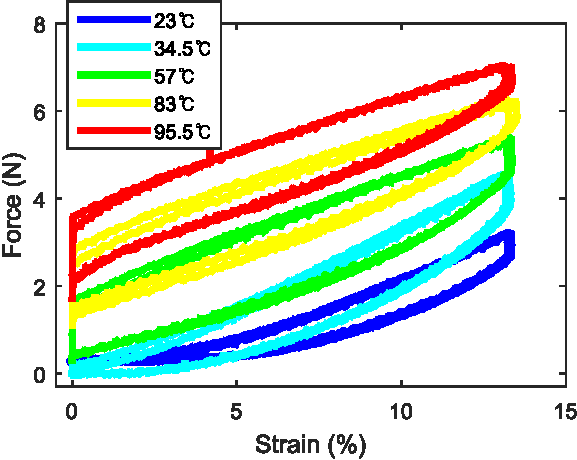
\includegraphics[width=\textwidth]{ForceStrain-cropped.pdf}
		\caption{\label{static1_result}}
	\end{subfigure}
	~
	\begin{subfigure}[t]{0.32\textwidth}
		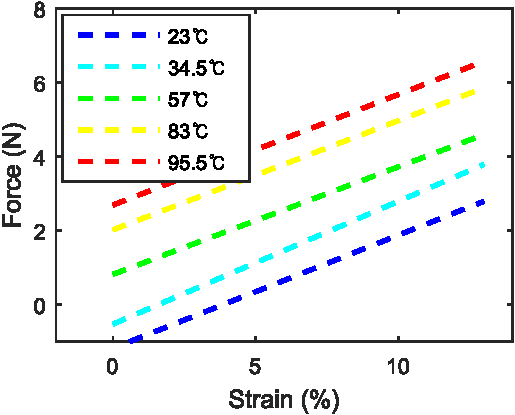
\includegraphics[width=\textwidth]{ForceStrain_line-cropped.pdf}
		\caption{\label{static1_line}}
	\end{subfigure}
	~
	\begin{subfigure}[t]{0.32\textwidth}
		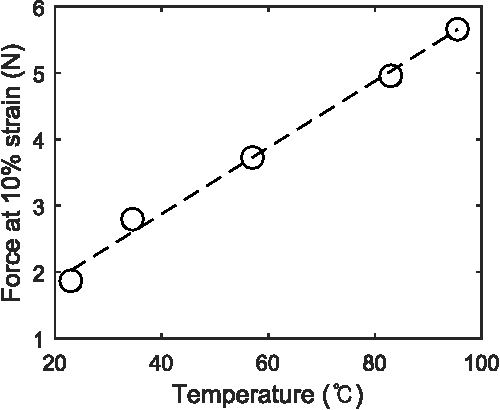
\includegraphics[width=\textwidth]{ForceStrain_dot-cropped.pdf}
		\caption{\label{static1_dot}}
	\end{subfigure}
	\caption[Results of the static experiment]{\subref{static1_result} Characteristic curves of \scp for various $T_{steady}$. \subref{static1_line} Linear graph of correlation between tension(force) and strain. \subref{static1_dot} Tension is linearly proportional to $T_{steady}$.}
	\label{static1_results}
\end{figure}

\subsection{Dynamic Experiment}\label{section_dynamic} % Important!!

The aim of the dynamic experiment was to verify the properties of \scps attributed by equation \eqref{thermo-electrical_model}, and to quantify the thermal conductivity of muscles by means of control of solenoid valve.
`Setup 2' was used for dynamic experiment, which was previously described in \ref{section_appa}. %TODO : 어색할수도

First, a constant power - which had varied over the experiments - was applied to the muscle.
The temperature of the muscle had increased exponentially and stopped increasing at specific point.
Also, by measuring the `steady temperature' $ T_{steady} $ at this `steady state' for 6 kinds of voltage, 
we could get Fig.\ref{powerdeltaT} and check that $ \Delta T $ is linearly proportional to power.
Therefore, these two properties of muscles verifies the equation \eqref{thermo-electrical_model}.

Second, the method for cooling the \scps are investigated and its performance was quantified. % TODO : 이 문단 조금 어색?
Since the amount of air flow couldn't be directly analog controlled,
it was done in digital way - it was periodically stopped and resumed.
This mechanism was performed by opening the solenoid valve in a constant ratio at each period. For example, if we make the valve be opened for \SI{70}{\milli\second} and closed for the next \SI{30}{\milli\second}, the ratio is 70\% in this situation. 
The ratio will be referred as `cooling ratio' and variable name $r$ will be used from henceforth.

The period of opening and closing was \SI{100}{\milli\second}, which was carefully chosen to achieve the best performance. If the period is too long, the thermal conductivity of the \scps will periodically change. On the other hand, if the period is too short, the solenoid valve won't perform well because it will take minimal time to open the valve. 

For this experiment, we carried out the following processes. We used constant voltage - \SI{2.59}{\volt}. Cooling ratio was variously changed, including $0$(Natural cooling, $\lambda_{N}$), and $1$(Complete forced cooling, $\lambda_{F}$). Also, five compressed air cans were implemented alternatively in order to maintain constant air pressure. 
\begin{enumerate}
	\item When the muscle became $T=T_{ambient}$, we started recording time and temperature.
	\item Constant power was applied until it reached the steady state.
	\item After reaching steady state, the power was disconnected and the cooling was started. 
	\item When the muscle's temperature reached $T=T_{ambient}$ again, we stopped recording. 
	\item We repeated the process 1-4 with other voltages and cooling ratios.
\end{enumerate}


\begin{figure}[t]
	\centering
	\begin{subfigure}[t]{0.45\linewidth}
		\centering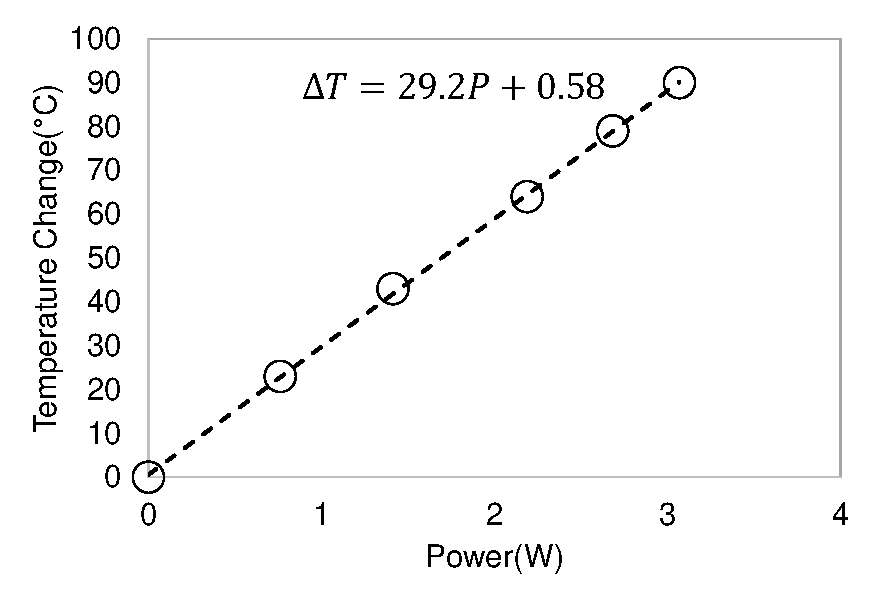
\includegraphics[width=\textwidth]{powerdeltaT-graph_v5.pdf}
		\caption{\label{powerdeltaT}}
	\end{subfigure}%
	\begin{subfigure}[t]{0.45\linewidth}
		\centering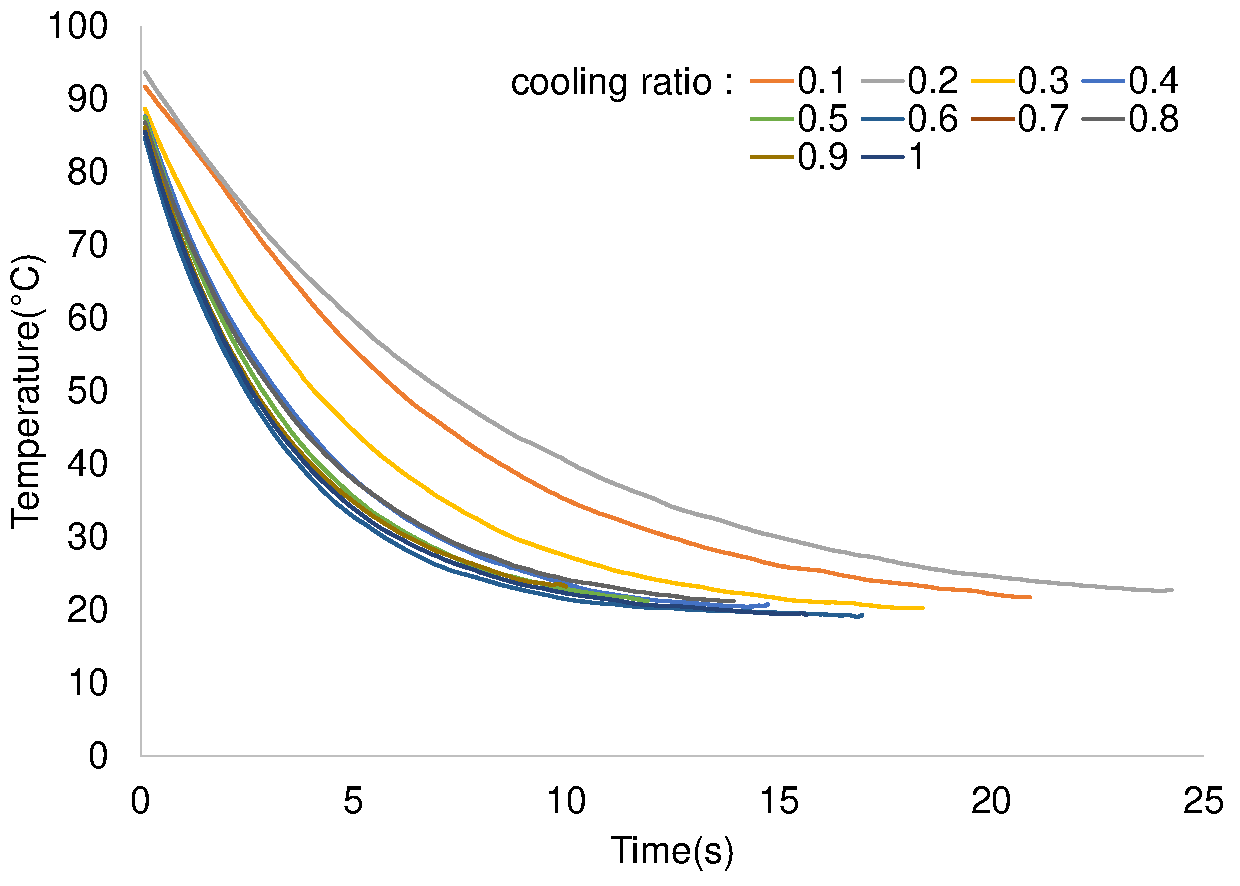
\includegraphics[width=\textwidth]{coolinggraph_v5.pdf}
		\caption{\label{coolinggraph}}
	\end{subfigure}
	\caption[Results of the dynamic experiment]{\subref{powerdeltaT} $ T_{steady} $ changes proportionally to power. \subref{coolinggraph} After power was shut down and forced cooling had began, temperature decreased exponentially.}
	\label{result_dynamic}
\end{figure}

First, by graphing the relation between power $P$ and temperature shift $\Delta{T}=T_{steady}-T_{ambient}$, we could check that they were linearly proportional as \eqref{dynamic_calculation_power}.
Also, we could find the fact that the temperature of \scp changes exponentially as shown in figure \ref{coolinggraph}. This was in line with  \eqref{thermo-electrical_model}.

\begin{equation} \label{dynamic_calculation_power}
P = \lambda\Delta{T}
\end{equation}
By applying \eqref{dynamic_calculation_power} to a heating graph, we could get $\lambda_{N}$ according to figure \ref{powerdeltaT}. Then, while calculating the time constant of the heating graph, we could calculate \scp system's specific heat $C_{th}$ with \eqref{dynamic_calculation_tau}.\footnote{This was measured three times, resulting \SI{51.3}{\second}, \SI{54.1}{\second}, and \SI{53.0}{\second}. The average value was \SI{52.8}{\second}.} 

\begin{equation}
\lambda_{N}=\SI{3.42e-2}{\watt\per\degreeCelsius}, C_{th}=\SI{1.81}{\joule\per\degreeCelsius}. \nonumber
\end{equation}
Now, we have the value of $C_{th}$, so the thermal conductivity can be obtained by using \eqref{dynamic_calculation_tau}. Analysis for each cooling graph is shown in figure \ref{analysis_dynamic}.

\begin{equation} \label{dynamic_calculation_tau}
\lambda = \frac{C_{th}}{\tau}
\end{equation}

\begin{figure}[t]
	\begin{subfigure}[t]{0.52\linewidth}
		\centering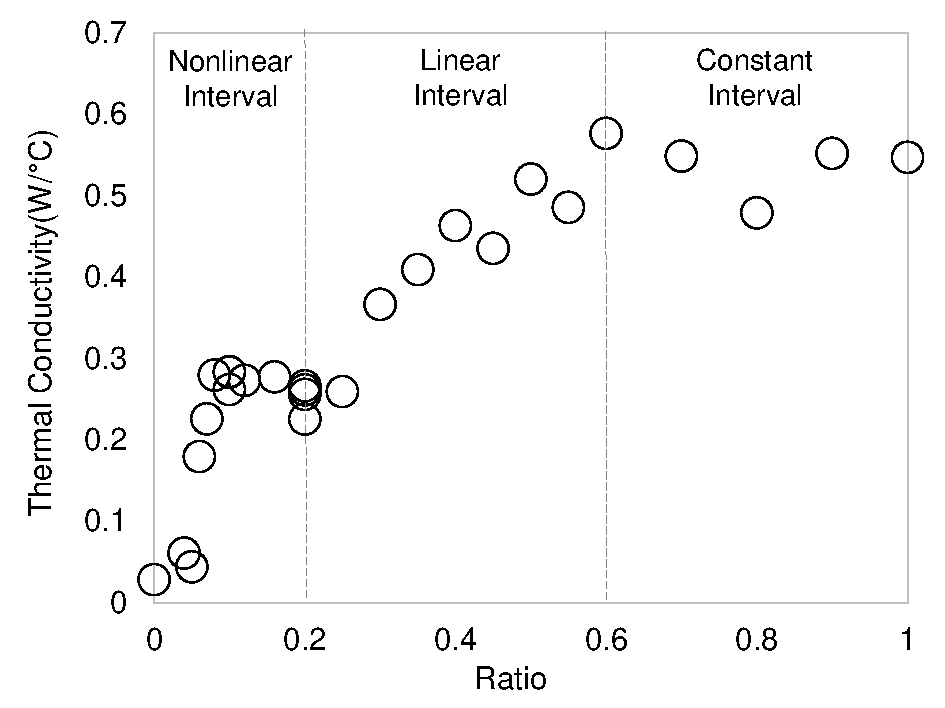
\includegraphics[width=\textwidth]{intervals_v3.pdf}
		\caption{\label{dynamic_proportional}}
	\end{subfigure}%
	\begin{subfigure}[t]{0.39\linewidth}
		%TODO : error - svg file not found...ㅠㅠ
		%\centering\includesvg[width=\textwidth]{../images/example}
		\centering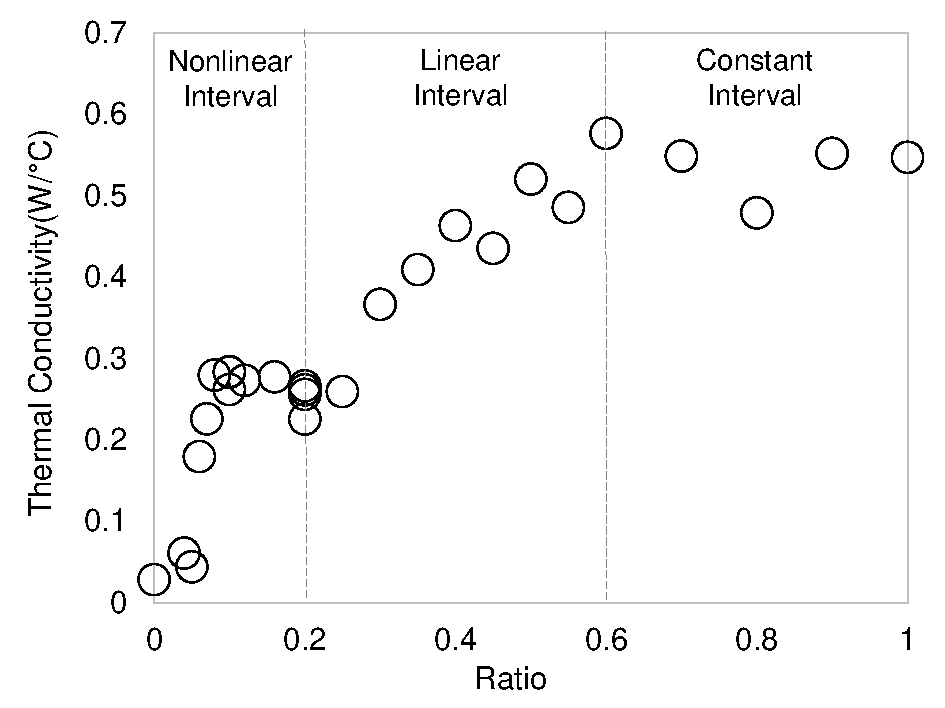
\includegraphics[width=\textwidth]{intervals_v3.pdf}
		\caption{\label{linear_interval}}
	\end{subfigure}
	\caption[Analysis of the dynamic experiment]{\subref{dynamic_proportional} $\lambda$ was linearly proportional to cooling ratio $r$ when $0.2<r<0.6$.  \subref{linear_interval} $\lambda$ could be calculated with the equation \eqref{lambda_control}.}
	\label{analysis_dynamic}
\end{figure}

In figure \ref{dynamic_proportional}, we can observe that the thermal conductivity in function of $r$ can be divided into three parts - nonlinear, linear, and constant interval. If $r<0.2$, $\lambda$ rapidly increased near $r=0.1$. Also, $\lambda$ wasn't increased anymore if $r>0.6$, {\it i.e.} $\lambda = \lambda_{F}$. This can be also observed from the cooling graph in figure \ref{coolinggraph}.
Therefore, the linear interval was chosen for the \Apcnospace.(Figure \ref{linear_interval}) The thermal conductivity in controllable(linear) interval was usually higher than cooling by computer fans, which were used by Yip \etalspace \cite{yip} and determined to be $\lambda_{fan}=\SI{0.30}{\watt\per\degreeCelsius}$.
\footnote{
	Meanwhile, we had to check that the load used in the dynamic experiment didn't affect muscle's thermal power. 
	Total electrical power of muscle was about $(\SI{1.0}{\volt})^2/(\SI{2.5}{\ohm})=\SI{0.4}{\watt}$, and cooling speed was about $\SI{1.39}{\joule\per\degreeCelsius} \cdot \SI{1}{\degreeCelsius\per\second}=\SI{1.39}{\watt}$ while gravitational power was about  $\SI{0.4}{\kilo\gram} \cdot  \SI{9.8}{\meter\per\second\square} \cdot \SI{0.001}{\meter\per\second}=\SI{0.004}{\watt}$. So we concluded that the load didn't affect the measurement of muscle's thermal properties.
}

\begin{equation} \label{lambda_control}
\lambda = 0.77\cdot r + 0.10 (\si{\watt\per\degreeCelsius}), 0.2\leq r \leq 0.6.
\end{equation}


\subsection{\APC Demonstration}

%\tocless \subsubsection{Demonstration - Two Period Sin Wave}
First, we demonstrated open-loop control of cooling speed by trying two-period sin wave control. In this demonstration, cooling was done during $t=$ \SI{40}{\second} - \SI{50}{\second}.\footnote{This slightly differs from the Table \ref{table_apc_sustain}.} To cool as much as possible, muscle 2 was cooled for all the time, and muscle 1 was `weakly' cooled by repeatedly opening and closing the solenoid valve. As a result, we got an rms error 26.6\% for the open-loop control, and 6.7\% for the closed-loop control.(Figure \ref{sustain_demo})

%After the demonstration, we concluded that an appropriate time for cooling will be \SI{30}{\second}-\SI{40}{\second}, not \SI{40}{\second} - \SI{50}{\second}. It is because 
\begin{figure}[t]
	\centering
	\begin{subfigure}[t]{0.45\textwidth}
		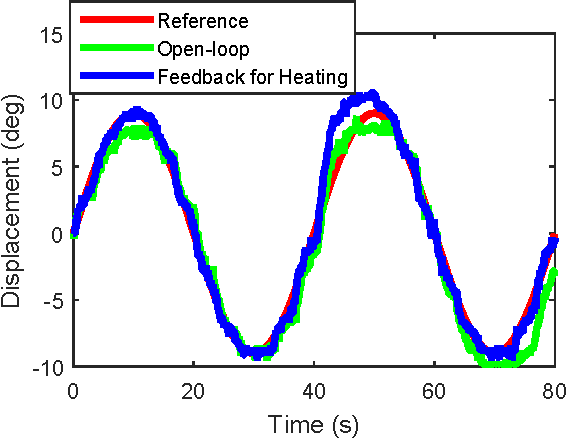
\includegraphics[width=\textwidth]{SinWave_cooling-cropped.pdf}
		\caption{\label{SinWave_cooling}}
	\end{subfigure}
	~
	\begin{subfigure}[t]{0.44\textwidth}
		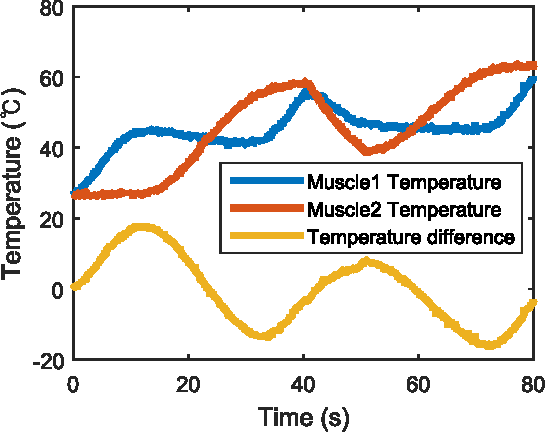
\includegraphics[width=\textwidth]{SinWaveC_T-cropped.pdf}
		\caption{\label{Sinwave_C_T}}
	\end{subfigure}
	\caption[Sustainable open-loop \apc demonstration.]{\subref{SinWave_cooling} Arm's angle in function of time. \subref{Sinwave_C_T} Temperature of two muscles in function of time. We checked that sustainable \apc was possible by cooling for some time.}
	\label{sustain_demo}
\end{figure}

%\tocless \subsubsection{Simulation - Feedback Control of Thermal Conductivity}


Integrating \eqref{dynamic_calculation_tau} and \eqref{lambda_control}, \eqref{tau_modification} was gained.
\begin{equation} \label{tau_modification} 
\begin{aligned} 
\tau & = \frac{C_{th}}{\lambda} \\
& = \frac{1.81}{0.77\cdot r + 0.10}. \\ 
\end{aligned}
\end{equation}
Also, by differentiating \eqref{simple_assume} and \eqref{theta_ref} with respect to time, \eqref{theta_diff} was drawn, where $t$ refers to time elapsed since $t=\SI{30}{\second}$.

\begin{equation} \label{theta_diff}
\begin{aligned} 
\frac{d\theta}{dt} & = \frac{c}{2kr}\cdot\frac{d}{dt}(T_{1}-T_{2}) \\
& = 9^{\circ}(2\pi\cdot 0.025)\sin{2\pi\cdot 0.025t}.
\end{aligned}
\end{equation}
What we had to do was to decrease $(T_{1}+T_{2})/2$, so \eqref{diff_t1+t2} was used. Constant $\alpha$ was carefully determined by several simulations.
\begin{equation} \label{diff_t1+t2}
\frac{d}{dt}(T_{1}+T_{2}) = -\alpha(T_{1}+T_{2}-2T_{ambient})
\end{equation}
Therefore, by using \eqref{thermo-electrical_model} for the each muscle, $\lambda_{1}$ and $\lambda_{2}$ need to be calculated. The block diagram which represents feedback control of thermal conductivities is shown in figure \ref{diagram_sustainable}.

\begin{figure}[t]
	\centering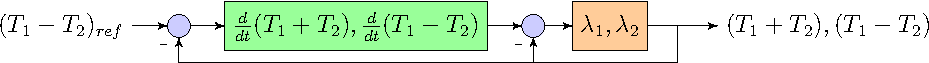
\includegraphics[width=\textwidth]{Diagram(v4)_sustainable.pdf}
	\caption{Block diagram for the sustainable \apcnospace.}
	\label{diagram_sustainable}
\end{figure}

To make sustainable \apc possible, $\lambda$ must be between $\SI{0.25}{\watt\per\degreeCelsius}$ and $\SI{0.60}{\watt\per\degreeCelsius}$  all the time, according to \eqref{lambda_control}. Therefore, possibility of this control strategy was verified by thermal simulation.
%We can guess that $\lambda_{1}$ have to decrease and $\lambda_{2}$ have to increase. 

Thermal conductivity of two muscles - $\lambda_{1}$ and $\lambda_{2}$ must hit its limit as late as possible. 
This duration was determined by constant $\alpha$ in \eqref{diff_t1+t2}. 
In figure \ref{Sinwave_C_T}, we observed that two of the muscles' average temperatures had increased approximately \SI{30}{\degreeCelsius}. This means that we had to cool down the average temperature at least \SI{30}{\degreeCelsius}. 
But, this optimization couldn't be solved algebraically, so it was solved by numerical simulation.
Simulation was carefully done by applying \eqref{thermo-electrical_model} and \eqref{EqAnta}, using the constants we got in section \ref{subsection_static_experiment}. The 4th order Runge-Kutta method was used to solve the differential equation. 

Through several simulations, we have concluded that $\alpha = 0.25$ is the best. The result of simulation with this value is shown in figure \ref{cool_simulation}. With initial temperature from figure \ref{Sinwave_C_T}, {\it i.e.} $T_{1}=\SI{40}{\degreeCelsius}$ and $T_{2}=\SI{55}{\degreeCelsius}$ at $t=\SI{30}{\second}$, the required thermal conductivity slightly hit the maximum limit. Also, the average temperature didn't decrease over \SI{30}{\degreeCelsius}. Therefore, the temperature would increase in this state.

Once average temperature increases, it will be easier to cool the muscles because $dT/dt \propto (T-T_{amb})$. Simulation was repeated with initial temperature $T_{1}=\SI{85}{\degreeCelsius}$ and $T_{2}=\SI{100}{\degreeCelsius}$ at $t=\SI{30}{\second}$. With those initial conditions, there was a dramatic decrease of average temperature. (Figure \ref{cool_control_100}) Also, required thermal conductivity hit the limit after cooling two of the muscles in full degree. 

After reaching the desired amount of cooling, $ \theta $ can be maintained as $\theta_{ref}$ by switching cooling to heating. Finally, we concluded that feedback cooling control is possible, so that we were able to make \apc highly sustainable.

\begin{figure}[t]
	\centering
	\begin{subfigure}[t]{0.45\textwidth}
		\centering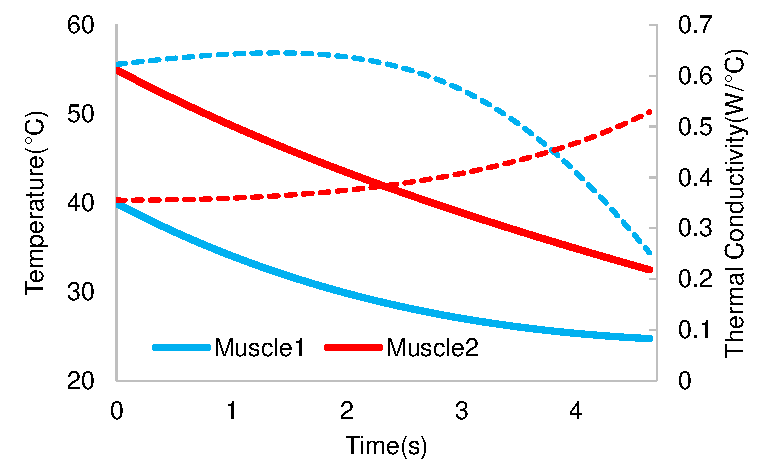
\includegraphics[width=\textwidth]{cool_control_T+lambda_v2.pdf}
		\caption{\label{cool_control}}
	\end{subfigure}%
	\begin{subfigure}[t]{0.45\textwidth}
		\centering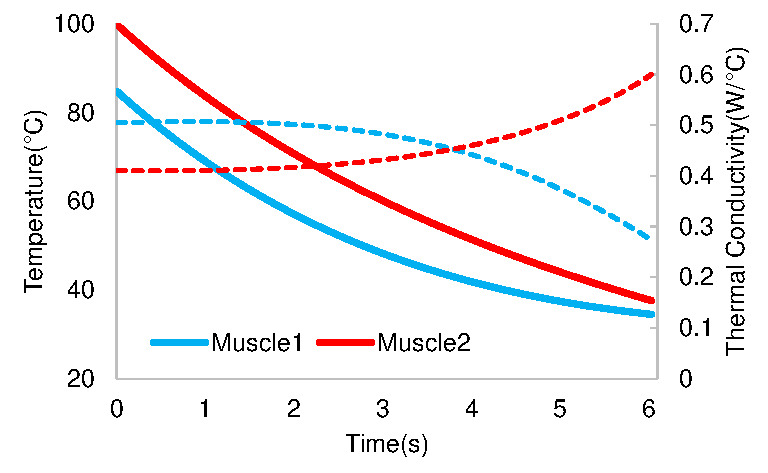
\includegraphics[width=\textwidth]{cool_control_T+lambda_100_85_v2.pdf}
		\caption{\label{cool_control_100}}
	\end{subfigure}
	\caption[Sustainable closed-loop \apc simulation]{\subref{cool_control} Temperature and thermal conductivity of two muscles in function of time after $t=\SI{30}{\second}$. Temperature is in full lines, and thermal conductivity is in broken lines. \subref{cool_control_100} Thermal conductivity of two muscles in function of time. }
	\label{cool_simulation}
\end{figure}




